% ============================================================
% CHAPTER 14 — PACK-LEVEL ESTIMATION AND CELL BALANCING
% ============================================================

\chapter{Pack-Level Estimation and Cell Balancing Architectures}
\label{ch:pack_level}

\section{Introduction: Beyond the Single Cell}
\label{sec:14_intro}

The estimation techniques developed in Chapters~5 through~9—ranging from Recursive Least Squares to the Extended Kalman Filter (EKF)—and the aging models of Chapter~13 were all derived under a fundamental constraint: the \textbf{single-cell assumption}. We treated the battery as a solitary electrochemical unit with a unified state of charge (SOC), a single terminal voltage, and a uniform core temperature.

In a production electric vehicle or grid-storage system, this assumption immediately breaks down. A high-voltage traction battery is not a single cell; it is a complex topology of hundreds or thousands of individual cells connected in series and parallel combinations. While the cells are manufactured to identical specifications, they do not behave identically in the real world. Two cells taken from the same production lot, installed in the same module, and cycled under the same nominal profile will diverge measurably within a few hundred cycles — a phenomenon commonly referred to as \emph{cell divergence} or \emph{pack fragmentation}.

This chapter addresses the computational and hardware architectures required to manage multi-cell packs. We will explore the physical origins of cell divergence, the algorithmic strategies to scale SOC/SOH estimation without exceeding microcontroller limits, the hardware balancing circuits required to correct imbalances before they degrade the entire pack, and the system-level trade-offs that govern real production designs. By the end of the chapter, the reader should be equipped to reason not only about \emph{how} a single cell is estimated, but about \emph{how that estimate is generalized, distributed, and corrected} across an entire energy storage system.

\subsection{Why Pack-Level Thinking Changes the Problem}
\label{subsec:14_why_pack}

It is tempting to think of pack-level management as "the same algorithm, just repeated many times." This intuition is incorrect for three separate reasons:

\begin{enumerate}
    \item \textbf{Computational scaling.} As shown in Section~\ref{sec:14_bar_delta}, naively replicating a full-order EKF for every cell scales computational cost combinatorially with pack size, quickly exceeding the throughput of an automotive-grade microcontroller.
    \item \textbf{Observability constraints.} In many production packs, only a subset of cell voltages are measured directly (some designs measure voltage at the module level rather than the cell level to save on wiring harness cost), meaning that individual cell states are not always fully observable.
    \item \textbf{Emergent failure modes.} Imbalance is not merely an estimation inconvenience — it is a safety-critical phenomenon. An undetected weak cell can be driven into over-voltage or over-discharge conditions even while the pack average appears nominal, potentially triggering thermal runaway.
\end{enumerate}

These three factors motivate the specialized architectures discussed throughout this chapter.

% ============================================================
\section{The Origins of Cell Imbalance}
\label{sec:14_imbalance}

If a pack consists of 100 cells in series (a typical 400~V architecture), the total pack capacity is governed by the weakest cell, and the total pack voltage is the sum of the individual cell voltages. Imbalance between these cells is driven by several interacting factors, which we now examine in detail.

\subsection{Manufacturing Tolerances}
\label{subsec:14_manufacturing}

Despite rigorous quality control, microscopic variations in electrode coating thickness, electrolyte volume, calendaring pressure, and internal tab welding result in a normal distribution of initial capacities ($Q_n$) and ohmic resistances ($R_0$) straight off the assembly line. A variance of 1\% to 2\% in baseline capacity is common and unavoidable in mass production, even among cells drawn from the same manufacturing batch and coating roll.

This variance is not static. Cell manufacturers typically grade cells into capacity "bins" (e.g., $\pm 0.5\%$, $\pm 1\%$, $\pm 2\%$) before shipment, and pack integrators will generally sort cells so that a single series string uses cells from a similar bin. However, binning at the time of manufacture only controls for the \emph{initial} condition — it says nothing about how two nominally identical cells will age under different local conditions inside the finished pack. In practice, even a perfectly sorted string of cells will diverge over time due to the mechanisms discussed below.

\subsection{Thermal Gradients and Arrhenius Aging}
\label{subsec:14_thermal}

As discussed in Chapter~13, cell degradation is highly sensitive to temperature. In a densely packed battery module, cells in the geographic center of the module have less surface area exposed to cooling channels than edge cells. Consequently, core cells operate at higher average temperatures.

\begin{figure}[htbp]
\centering
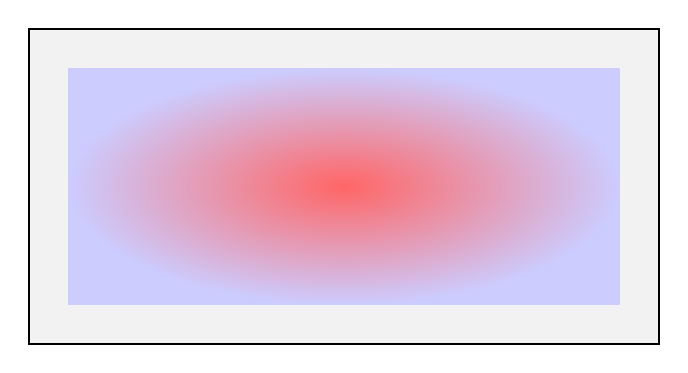
\begin{tikzpicture}
    % Placeholder for thermal gradient image
    \draw[thick, fill=gray!10] (0,0) rectangle (8,4);
    \node[align=center] at (4,2) {[\textit{Thermal Imaging Placeholder}] \\ Core cells show $T \approx 45^\circ$C \\ Edge cells show $T \approx 35^\circ$C};
    % Gradient illustration
    \shade[inner color=red!60, outer color=blue!20] (0.5,0.5) rectangle (7.5,3.5);
\end{tikzpicture}
\caption{Thermal gradients drive uneven aging rates across a battery module.}
\label{fig:14_thermal_gradient}
\end{figure}

Because Solid Electrolyte Interphase (SEI) layer growth accelerates exponentially with temperature (following Arrhenius kinetics), the hotter core cells experience faster capacity fade and resistance growth over months of cycling. As the $R_0$ of a core cell increases, it generates more $I^2 R_0$ Joule heating during operation, creating a positive feedback loop that accelerates its aging even further compared to its cooler neighbors.

This feedback loop can be expressed approximately as a coupled pair of differential relationships:
\begin{equation}
    \frac{dR_{0,i}}{dt} \propto A \, e^{-E_a / (k_B T_i)}, \qquad
    T_i \propto T_{\text{ambient}} + I^2 R_{0,i}(t) \cdot \theta_{\text{thermal}}
    \label{eq:14_thermal_feedback}
\end{equation}
where $E_a$ is the activation energy of the dominant degradation mechanism, $k_B$ is Boltzmann's constant, and $\theta_{\text{thermal}}$ is the thermal resistance between the cell core and the coolant. Equation~\ref{eq:14_thermal_feedback} illustrates why a pack with poor thermal uniformity will show \emph{accelerating}, not merely additive, divergence over its service life — a small initial temperature delta of 5–10$^\circ$C between core and edge cells can compound into a 2--3$\times$ difference in resistance growth rate after several thousand cycles.

\subsection{Non-Uniform Current Distribution in Parallel Groups}
\label{subsec:14_parallel_current}

A frequently overlooked source of imbalance occurs within parallel-connected cell groups (the "P" in a series-parallel, or "sXpY," pack architecture). Even though cells within a parallel group are electrically tied at both terminals, differences in busbar length, weld resistance, and local impedance mean that current does not divide evenly among them. A cell with a marginally lower internal resistance, or one positioned closer to the current collector tab, will carry a disproportionate share of the group's current. Over time this current asymmetry produces the same divergence in capacity and resistance seen across series strings, but it is far harder to detect because parallel-group cells are usually not individually instrumented — the BMS typically measures only the combined voltage and current of the group.

\subsection{Connection and Interconnect Resistance}
\label{subsec:14_interconnect}

Busbar welds, laser-welded tabs, and connector crimps each introduce a small but non-negligible resistance, typically on the order of 0.1–1~m$\Omega$. Manufacturing variance in weld quality means these interconnect resistances are themselves randomly distributed across the pack. Because interconnect resistance adds directly to the apparent $R_0$ of a cell as seen by the BMS, poorly characterized interconnects can be mistaken for genuine cell-level aging, leading estimation algorithms to misattribute capacity fade to the electrochemical cell when the real cause is a degrading mechanical joint (a failure mode sometimes accelerated by vibration and thermal cycling in vehicle applications).

\subsection{Self-Discharge Rate Variation}
\label{subsec:14_self_discharge}

All electrochemical cells exhibit some rate of self-discharge, driven by parasitic side reactions and micro-scale internal shorting from lithium plating or separator defects. While typical self-discharge rates are small (often under 2\% per month), the rate itself varies from cell to cell, and cells with elevated self-discharge — sometimes an early indicator of a latent manufacturing defect — will silently drift toward a lower SOC than their neighbors during long rest periods (e.g., a vehicle parked for several weeks). Because this divergence occurs while the pack is idle and unmonitored by an active estimation loop, it is one of the more difficult imbalance sources to detect proactively, and is a major reason production BMS designs specify periodic "wake and check" balancing cycles even when the vehicle is not in use.

\subsection{Cumulative Effect Over Pack Lifetime}
\label{subsec:14_cumulative}

Table~\ref{tab:14_imbalance_sources} summarizes the dominant imbalance mechanisms discussed above, their typical time constants, and their relative severity in production packs.

\begin{table}[htbp]
\centering
\caption{Summary of cell imbalance mechanisms in multi-cell packs.}
\label{tab:14_imbalance_sources}
\renewcommand{\arraystretch}{1.4}
\begin{tabularx}{\textwidth}{@{}l X X@{}}
\toprule
\textbf{Mechanism} & \textbf{Typical Time Constant} & \textbf{Detectability} \\
\midrule
Manufacturing tolerance & Present from day one (static) & High (factory test data) \\
Thermal gradient aging & Weeks to months (cumulative) & Medium (requires thermal + aging model) \\
Parallel-group current skew & Months (cumulative, self-masking) & Low (not individually instrumented) \\
Interconnect resistance drift & Months to years & Low (confounded with cell $R_0$) \\
Self-discharge variation & Days to weeks (during rest) & Low (requires long-rest voltage logging) \\
\bottomrule
\end{tabularx}
\end{table}

No single mechanism dominates in every application; a grid-storage system sitting at a fixed ambient temperature will be dominated by manufacturing tolerance and self-discharge effects, while a high-power EV pack undergoing aggressive fast-charging cycles will be dominated by the thermal feedback loop of Section~\ref{subsec:14_thermal}. A robust BMS design must therefore budget balancing hardware capacity and estimation bandwidth for the \emph{worst-case combination} of these effects, not merely the average case observed in early validation testing.

% ============================================================
\section{Pack Topology and Its Effect on Estimation}
\label{sec:14_topology}

Before addressing estimation algorithms directly, it is useful to review how pack topology constrains what can actually be measured and, therefore, what can be estimated.

\subsection{Series-Only vs. Series-Parallel Architectures}
\label{subsec:14_series_parallel}

A purely series ("Ns") architecture places every cell in a single current path, meaning every cell carries identical current at every instant. This simplifies estimation because the input $I$ to every cell-level model is shared and known exactly. Most modern EV packs, however, use a series-parallel ("NsPy") architecture, in which $y$ cells are grouped in parallel to form a single "brick," and $N$ such bricks are placed in series to reach the desired pack voltage. This is done primarily to reach the required pack energy and power without requiring individual cells of impractically large format.

The series-parallel topology introduces the parallel-current-skew problem discussed in Section~\ref{subsec:14_parallel_current}, and, more importantly for estimation, it usually means the BMS can only measure the combined terminal voltage of the brick, not the voltage of each cell within it. This has a direct consequence: \emph{the finest granularity of estimation achievable by the BMS is generally the granularity of the finest granularity of measurement available to it.} A pack instrumented at the brick level can only ever estimate brick-level SOC and SOH; individual cell-level divergence within a brick can only be inferred indirectly (for example, via impedance spectroscopy at production test, or by post-mortem teardown), not tracked online.

\subsection{Sensing Architecture: Centralized vs. Modular BMS}
\label{subsec:14_sensing_arch}

Two dominant sensing architectures exist in production:

\begin{itemize}
    \item \textbf{Centralized BMS:} A single controller directly wires to every cell tap in the pack via a large wiring harness. This architecture offers the lowest latency and the simplest software model but does not scale well beyond a few dozen cells due to harness weight, connector count, and EMI susceptibility.
    \item \textbf{Modular (Daisy-Chained) BMS:} Each module contains its own local cell-monitoring IC, which measures voltages and temperatures for the cells in that module and communicates upstream to a pack-level controller over an isolated serial bus (commonly a proprietary isoSPI or similar differential link). This is the dominant architecture in modern EVs, as it dramatically reduces harness complexity.
\end{itemize}

The modular architecture introduces an additional practical constraint that is easy to overlook in a purely algorithmic treatment: \emph{communication latency and jitter}. In a daisy chain of, say, 12 modules, the last module's voltage reading may be sampled several milliseconds after the first module's reading. For a pack-average EKF running at 10~Hz, this skew is negligible; but for delta-observer designs intended to catch fast transient divergence (for example, detecting an internal short in real time), the designer must explicitly account for inter-module sampling skew or risk misattributing a timing artifact to a genuine cell fault.

% ============================================================
\section{Pack-Level State Estimation: The ``Bar-Delta'' Approach}
\label{sec:14_bar_delta}

The most naive approach to pack-level estimation is to duplicate the single-cell EKF architecture for every cell in the pack. However, as established in the computational cost analysis of Chapter~11, the matrix inversions required for an EKF scale cubically, $\mathcal{O}(n^3)$, in the dimension of the state vector, and the wall-clock cost of running $N$ independent filters scales linearly in $N$ on top of that. Running 100 independent EKFs at 10~Hz is computationally prohibitive for standard automotive microcontrollers, which are typically constrained to a small fraction of a modern desktop CPU's floating-point throughput and must reserve the majority of their cycles for safety-critical control loops, CAN communication, and diagnostic monitoring.

To solve this, modern Smart-BMS architectures employ \textbf{Difference Filtering} (often called the Bar-Delta approach). Instead of treating every cell as an independent system, the BMS assumes that all cells follow a similar baseline trajectory, with minor individual deviations.

\subsection{Architecture Overview}
\label{subsec:14_bar_delta_overview}

\begin{enumerate}
    \item \textbf{The ``Bar'' Filter (Pack Average):}
    A single, full-order Extended Kalman Filter is run to estimate the average state of the pack, $\bar{x}$. This filter uses the average terminal voltage $\bar{V}_t$ and the common series current $I$. It maintains the heavy computational matrices for the nominal pack SOC and polarization voltages.

    \item \textbf{The ``Delta'' Filters (Cell Deviations):}
    For each individual cell $i$, a highly simplified, low-order observer (such as a Proportional-Integral observer or a 1D Kalman Filter) tracks only the \emph{deviation} from the pack average:
    \begin{equation}
        \Delta x_i = x_i - \bar{x}
        \label{eq:14_delta_x}
    \end{equation}
\end{enumerate}

Because $\Delta x_i$ changes very slowly (cells drift apart over weeks, not milliseconds), the delta filters can be updated at a much slower rate (e.g., 0.1~Hz) and require minimal matrix math. The absolute state of any specific cell is then easily reconstructed as:
\begin{equation}
    x_i = \bar{x} + \Delta x_i
    \label{eq:14_reconstruct_x}
\end{equation}
This architecture reduces the computational load by orders of magnitude while preserving individual cell visibility.

\subsection{Formal Derivation of the Delta Dynamics}
\label{subsec:14_delta_derivation}

To understand why the delta filter can be so much simpler than the bar filter, it is instructive to derive its governing equation explicitly. Consider the standard single-cell equivalent-circuit model used throughout Chapters~5–9, in discrete time:
\begin{align}
    z_i[k+1] &= z_i[k] - \frac{\eta \, \Delta t}{Q_{n,i}} I[k] \label{eq:14_soc_update}\\
    V_{t,i}[k] &= V_{oc}(z_i[k]) - I[k] R_{0,i} - V_{p,i}[k]
    \label{eq:14_voltage_model}
\end{align}
where $z_i$ is the SOC of cell $i$, $Q_{n,i}$ is its capacity, $R_{0,i}$ its ohmic resistance, and $V_{p,i}$ its polarization voltage. Define the pack-average quantities $\bar{z}$, $\bar{Q}_n$, and $\bar{R}_0$ as the arithmetic means across all $N$ cells. Subtracting the pack-average version of Equation~\ref{eq:14_soc_update} from the cell-specific version and linearizing the $1/Q_{n,i}$ term around $\bar{Q}_n$ yields, to first order:
\begin{equation}
    \Delta z_i[k+1] \approx \Delta z_i[k] - \frac{\eta \, \Delta t \, I[k]}{\bar{Q}_n^2}\, \Delta Q_{n,i}
    \label{eq:14_delta_soc_update}
\end{equation}
where $\Delta Q_{n,i} = Q_{n,i} - \bar{Q}_n$ is treated as a slowly time-varying (near-constant) parameter rather than a fast state. The key structural insight is that Equation~\ref{eq:14_delta_soc_update} is linear and driven by a single scalar parameter deviation, in contrast to the full nonlinear model of Equation~\ref{eq:14_soc_update}, which must track the open-circuit voltage curve, polarization dynamics, and capacity simultaneously. This is precisely why a first-order or PI-style observer suffices at the delta level: the nonlinear "heavy lifting" has already been absorbed by the bar filter, and the delta filter need only track a small, approximately linear residual.

\subsection{Observability and Tuning Considerations}
\label{subsec:14_observability}

The Bar-Delta architecture is not free of subtlety. Two practical issues deserve attention:

\begin{itemize}
    \item \textbf{Observability of $\Delta z_i$ from voltage alone.} Since only $\Delta V_{t,i}$ is directly measured, and the mapping from $\Delta z_i$ to $\Delta V_{t,i}$ depends on the local slope of the open-circuit voltage curve $dV_{oc}/dz$, cells operating on the flat plateau region of the OCV curve (common in LFP chemistries) exhibit poor observability of $\Delta z_i$ from voltage measurements. In these operating regions, the delta filter should rely more heavily on the coulomb-counting term of Equation~\ref{eq:14_delta_soc_update} and reduce its gain on the voltage-innovation term, or, more robustly, the BMS should schedule a periodic rest period at a steep region of the OCV curve purely to re-anchor the delta estimates.
    \item \textbf{Filter divergence under aggressive load transients.} Because the delta filter update rate is deliberately slow (0.1~Hz in the nominal design), an abrupt, large disturbance to a single cell — for instance, a partial internal short — may not be corrected quickly enough by the delta filter alone. Production designs typically supplement the Bar-Delta architecture with a fast, threshold-based hardware comparator that monitors raw cell voltage independently of the estimation software, providing a redundant, low-latency safety trip that does not depend on filter convergence.
\end{itemize}

\subsection{Computational Savings in Practice}
\label{subsec:14_savings}

Table~\ref{tab:14_computation_savings} presents an approximate comparison of the computational load between the naive per-cell EKF approach and the Bar-Delta approach, for a representative 96-cell series pack.

\begin{table}[htbp]
\centering
\caption{Approximate computational load comparison for a 96-cell pack.}
\label{tab:14_computation_savings}
\renewcommand{\arraystretch}{1.4}
\begin{tabularx}{\textwidth}{@{}l X X@{}}
\toprule
\textbf{Architecture} & \textbf{Filters Required} & \textbf{Relative FLOP Load} \\
\midrule
Naive (96 independent EKFs, 3-state) & 96 full EKFs @ 10~Hz & $\sim$96$\times$ baseline \\
Bar-Delta (1 EKF + 96 delta observers) & 1 full EKF @ 10~Hz + 96 1D observers @ 0.1~Hz & $\sim$1.1$\times$ baseline \\
\bottomrule
\end{tabularx}
\end{table}

This roughly two-order-of-magnitude reduction is what makes real-time, cell-resolved SOC and SOH estimation tractable on a cost-constrained automotive microcontroller, and it is the primary reason the Bar-Delta family of architectures (and its many commercial variants) has become the de facto standard across the industry.

% ============================================================
\section{Alternative and Complementary Estimation Strategies}
\label{sec:14_alternatives}

While Bar-Delta filtering is the dominant production architecture, it is worth briefly surveying alternative approaches that appear in the literature and in specialized applications, as they illuminate different trade-offs.

\subsection{Clustering-Based Estimation}
\label{subsec:14_clustering}

Rather than modeling every cell individually, a clustering approach groups cells into a small number of "representative" bins (e.g., 3–5 clusters) based on similarity in voltage response, and runs a full-order filter for each cluster rather than for each cell. This offers a middle ground between the single bar filter and full per-cell estimation, and is particularly attractive in packs with a bimodal or multimodal degradation pattern — for example, a pack where cells in a single hot corner age distinctly differently from the rest of the pack, such that a single "average" bar filter poorly represents either population.

\subsection{Distributed (Consensus) Kalman Filtering}
\label{subsec:14_distributed}

In modular BMS architectures where each module already contains a local microcontroller, it is possible to run a small local filter on each module and exchange only summary statistics (rather than raw voltage/current data) with neighboring modules or the pack-level controller, converging toward a consistent pack-wide estimate through a consensus algorithm. This approach reduces the communication bandwidth required across the daisy-chain bus at the cost of more complex convergence analysis and a coordination overhead that in most current-generation vehicle platforms outweighs its benefits — it remains primarily a topic of active research rather than a widely deployed production technique as of this writing.

\subsection{Data-Driven and Machine-Learning-Assisted Delta Prediction}
\label{subsec:14_ml_delta}

An emerging complement to the analytical delta observer of Section~\ref{sec:14_bar_delta} is to train a lightweight regression or gradient-boosted model offline, using historical fleet data, to \emph{predict} the expected $\Delta x_i$ trajectory for a cell given its position in the pack, its cumulative throughput, and its historical temperature exposure. Such a model does not replace the delta observer but can be used to provide a better prior, accelerating convergence after a BMS reset or a cold start, and can also flag cells whose observed deviation grows faster than the population-level model would predict — a useful early-warning indicator that a cell may be developing an incipient fault rather than merely exhibiting ordinary manufacturing-driven drift.

% ============================================================
\section{Cell Balancing Mechanisms}
\label{sec:14_balancing}

Estimation algorithms can identify which cells are drifting apart, but estimation alone cannot fix the physical imbalance. Because series-connected cells share the exact same current $I$, a cell with lower capacity will reach its maximum voltage cutoff before the rest of the pack, forcing the BMS to halt the charging process prematurely. To restore usable capacity, the BMS uses balancing circuits to equalize the cells.

\subsection{Passive Balancing (Dissipative)}
\label{subsec:14_passive}

Passive balancing is the industry standard due to its simplicity, low cost, and reliability. Each cell is wired in parallel with a bypass circuit consisting of a MOSFET switch and a shunt resistor.

When the BMS detects that a cell's voltage (or estimated SOC) is higher than the pack average, it closes the switch. The excess energy in that specific cell is bled off as heat through the resistor ($V^2/R$).
\begin{itemize}
    \item \textbf{Pros:} Cheap, small PCB footprint, highly reliable.
    \item \textbf{Cons:} Generates excess thermal load inside the battery pack; literally burns away usable energy; can generally only balance efficiently during the top-end of the charge cycle.
\end{itemize}

\subsubsection{Sizing the Balancing Resistor}
\label{subsubsec:14_resistor_sizing}

The choice of shunt resistor value is a direct trade-off between balancing speed and thermal load. The bleed current through the resistor is given by
\begin{equation}
    I_{\text{bleed}} = \frac{V_{\text{cell}}}{R_{\text{shunt}}}
    \label{eq:14_bleed_current}
\end{equation}
and the power dissipated, which must be managed by the module's thermal design, is
\begin{equation}
    P_{\text{dissipated}} = \frac{V_{\text{cell}}^2}{R_{\text{shunt}}}
    \label{eq:14_bleed_power}
\end{equation}
Typical production designs target a bleed current on the order of 50–150~mA per cell, corresponding to shunt resistor values in the range of 20–80~$\Omega$ for a nominal 3.6–4.2~V lithium-ion cell. Lower resistance values balance faster but require larger resistors (or multiple resistors in parallel) and more aggressive thermal management of the balancing PCB itself, which is often mounted in close thermal proximity to the very cells it is trying to protect from over-temperature.

\subsubsection{Balancing Duty Cycle and Duration}
\label{subsubsec:14_duty_cycle}

Because passive balancing current is small relative to the pack's charge or discharge current, meaningful correction of even a few percent of SOC imbalance can take several hours of continuous bleeding. This is one of the principal reasons production vehicles perform balancing predominantly while connected to shore power (AC charging) overnight, when the vehicle is stationary and time is abundant, rather than attempting to fully balance the pack during normal driving, where balancing current is a rounding error next to hundreds of amps of traction current.

\subsection{Active Balancing (Non-Dissipative)}
\label{subsec:14_active}

Active balancing attempts to achieve close to 100\% energy utilization. Instead of burning off the excess energy of the highest-charged cell as heat, active balancing circuits use inductors, switched capacitors, or DC-DC flyback transformers to shuttle charge from the strongest cells directly into the weakest cells.

\begin{itemize}
    \item \textbf{Pros:} Highly efficient, extends usable vehicle range, generates minimal heat, can balance dynamically during driving (discharge).
    \item \textbf{Cons:} Requires bulky magnetic components (inductors/transformers); significantly more expensive; higher risk of hardware failure.
\end{itemize}

\subsubsection{Switched-Capacitor Topologies}
\label{subsubsec:14_switched_cap}

In a switched-capacitor balancer, a capacitor is alternately connected across a higher-voltage cell and then across its lower-voltage neighbor, transferring a small packet of charge on each switching cycle. This topology is attractive because it requires no magnetic components and can be implemented with relatively inexpensive discrete switches, but it fundamentally only transfers charge between \emph{adjacent} cells, meaning imbalance correction between cells at opposite ends of a long series string must "ripple" cell-by-cell down the chain, which can be slow for large packs.

\subsubsection{Inductor-Based and Flyback Transformer Topologies}
\label{subsubsec:14_inductor}

Inductor-based balancers store energy from a high-voltage cell in a magnetic field during one switching phase and then release that energy into a target cell (or directly onto the pack bus) during the next phase. Multi-winding flyback transformer designs go further, allowing energy to be extracted from any single cell and delivered directly to the full pack bus (cell-to-pack balancing) or vice versa (pack-to-cell), removing the "adjacent cell only" limitation of the switched-capacitor approach at the cost of a more complex and more expensive magnetic component and driver circuit.

\subsubsection{Efficiency and Component Considerations}
\label{subsubsec:14_active_efficiency}

Reported round-trip efficiencies for active balancing hardware in the literature and in commercial datasheets typically fall in the 85–95\% range, with switched-capacitor designs at the lower end (due to resistive losses in the switches and ESR of the capacitors) and well-designed transformer-based topologies at the higher end. Even at 90\% efficiency, however, active balancing systems introduce non-trivial engineering overhead: the additional magnetic components add mass and volume that must be accommodated within the pack enclosure, the additional switching circuitry is itself a source of electromagnetic interference that must be managed for automotive EMC compliance, and the incremental bill-of-materials cost (often cited in industry teardown analyses as several times that of an equivalent passive balancing board) must be justified against the modest capacity gain it delivers.

\subsection{Comparative Summary}
\label{subsec:14_comparison_table}

\begin{table}[htbp]
\centering
\caption{System-level comparison of Active vs. Passive balancing architectures.}
\label{tab:14_balancing_comparison}
\renewcommand{\arraystretch}{1.4}
\begin{tabularx}{\textwidth}{@{}l X X@{}}
\toprule
\textbf{Metric} & \textbf{Passive Balancing} & \textbf{Active Balancing} \\
\midrule
\textbf{Energy Transfer} & Bleeds excess energy as heat. & Shuttles energy to weak cells. \\
\textbf{Efficiency} & Low ($\sim$0\% energy recovered). & High (85\%--95\% energy recovered). \\
\textbf{Thermal Output} & High (requires robust thermal management). & Very Low. \\
\textbf{Hardware Cost} & Low (Resistors and MOSFETs). & High (Transformers, inductors, complex ICs). \\
\textbf{Balancing Speed} & Slow (limited by bleed current, hours). & Moderate to fast, depending on topology. \\
\textbf{Balances During Driving?} & Generally limited to charge-only. & Yes, can balance during discharge. \\
\textbf{Primary Use Case} & Consumer EVs, power tools, grid storage. & Aerospace, racing, second-life batteries. \\
\bottomrule
\end{tabularx}
\end{table}

\begin{quote}
\textbf{Key insight:} While active balancing is mathematically and physically superior, the automotive industry overwhelmingly relies on passive balancing. The cost, weight, and volume penalties of active balancing hardware rarely justify the 2--3\% gain in pack capacity, except in specialized aerospace or second-life battery applications where aging divergence is extreme.
\end{quote}

% ============================================================
\section{Balancing Algorithms and Triggering Strategies}
\label{sec:14_balancing_algorithms}

Having the balancing hardware in place is only half of the design problem; the BMS must also decide \emph{when} and \emph{how aggressively} to balance. Poorly designed triggering logic can waste energy balancing cells that are within acceptable tolerance, or fail to balance cells that are diverging quickly enough to matter.

\subsection{Voltage-Based Triggering}
\label{subsec:14_voltage_trigger}

The simplest and most common strategy compares each cell's terminal voltage against the maximum (or minimum) voltage in the string and enables balancing for any cell exceeding a fixed threshold, typically on the order of 10–30~mV above the pack minimum during the top-of-charge region. This approach is computationally trivial and requires no model of the cell, but it is chemistry-dependent in its effectiveness: for chemistries with a steep OCV-SOC curve near full charge (e.g., NMC), a small voltage delta corresponds to a small SOC delta, making voltage-based triggering reasonably accurate. For flat-curve chemistries (e.g., LFP), the same voltage delta can correspond to a much larger, and more uncertain, SOC delta, reducing the reliability of pure voltage-based triggering.

\subsection{SOC-Based Triggering}
\label{subsec:14_soc_trigger}

A more sophisticated approach uses the delta-filter SOC estimates from Section~\ref{sec:14_bar_delta} directly, triggering balancing based on estimated $\Delta z_i$ rather than raw voltage. This decouples the balancing decision from the shape of the OCV curve and allows balancing to be intelligently scheduled even away from the top-of-charge plateau (for chemistries and duty cycles where this is desirable), at the cost of making the balancing system's correctness directly dependent on the accuracy of the underlying estimator.

\subsection{Predictive and Schedule-Aware Balancing}
\label{subsec:14_predictive_balancing}

Some production systems go further and incorporate predictive elements: rather than reacting only to the currently observed imbalance, the BMS uses the historical drift rate of each cell (tracked by the delta filter over previous charge cycles) to anticipate which cells are likely to require balancing during the \emph{next} charge event, and pre-emptively adjusts the charging profile (for example, by tapering current slightly earlier for a string containing a known fast-drifting cell) to reduce the total balancing burden and total energy wasted over the vehicle's lifetime, rather than optimizing purely for the current charge cycle in isolation.

% ============================================================
\section{Fault Detection and Safety Interlocks at the Pack Level}
\label{sec:14_fault_detection}

Pack-level estimation and balancing cannot be considered in isolation from the safety architecture that surrounds them, since an undetected imbalance is ultimately a safety hazard, not merely an efficiency concern.

\subsection{Redundant Voltage Monitoring}
\label{subsec:14_redundant_monitoring}

Given the safety stakes of over-voltage and under-voltage conditions at the individual cell level, production BMS designs virtually always implement a secondary, independent voltage monitoring path — often a separate, simpler ASIC dedicated purely to threshold comparison — that can trigger a contactor-opening safety response even if the primary estimation microcontroller has hung, crashed, or is otherwise producing unreliable state estimates. This redundancy principle should be understood as a complement to, not a replacement for, the estimation architectures discussed in this chapter: the Bar-Delta filter provides the nuanced, continuous state picture needed for performance and longevity optimization, while the independent hardware comparator provides the blunt, always-available safety backstop.

\subsection{Distinguishing Ordinary Drift from Incipient Faults}
\label{subsec:14_fault_vs_drift}

One of the more subtle responsibilities of the pack-level estimation layer is to distinguish between ordinary, expected cell-to-cell drift (as characterized in Section~\ref{sec:14_imbalance}) and the early signature of a genuine cell fault, such as an internal micro-short or separator defect. A useful heuristic, used in various forms across the industry, is to monitor the \emph{rate of change} of $\Delta x_i$ rather than its absolute magnitude: ordinary manufacturing- and thermal-driven drift accumulates gradually over many charge cycles, whereas an incipient internal fault typically produces a comparatively rapid and accelerating divergence, often accompanied by an anomalous self-discharge signature during rest periods (Section~\ref{subsec:14_self_discharge}). Flagging cells whose drift rate crosses a statistically-derived threshold (relative to the observed population distribution across the rest of the pack) allows the BMS to escalate specific cells for closer monitoring, or to schedule proactive service, well before the imbalance becomes severe enough to trip a hard safety limit.
\begin{figure}[H]
\centering
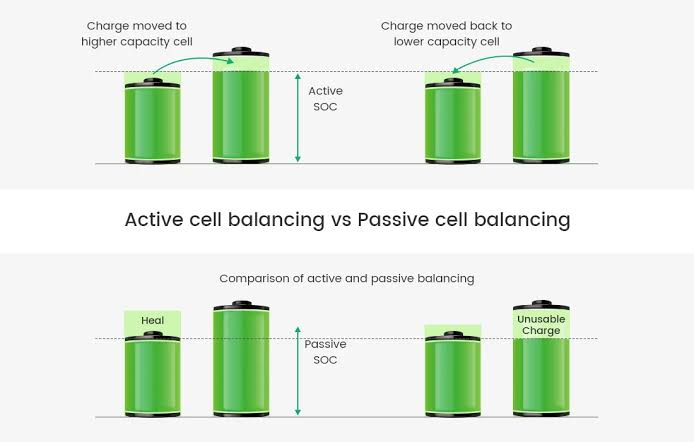
\includegraphics[width=0.65\textwidth]{chapter11-cell-balancing.jpg}
\caption{Active (shuttling) vs. Passive (bleeding) balancing}
\label{fig:cell_balancing_mechanisms}
\end{figure}

% ============================================================
\section{Summary}
\label{sec:14_summary}

Transitioning from a single-cell model to a multi-cell pack fundamentally shifts the bottleneck of battery management from pure algorithmic accuracy to computational scalability and hardware intervention. Manufacturing tolerances, thermal gradients, parallel-group current skew, interconnect resistance drift, and self-discharge variation all guarantee that cells will drift apart over their lifespan, and pack topology and sensing architecture determine the finest granularity at which this drift can even be observed.

To track this drift efficiently, the Bar-Delta estimation topology allows the BMS to monitor individual cell SOC and SOH without overwhelming the microcontroller, by combining a single full-order pack-average filter with a bank of lightweight, slowly-updated per-cell deviation observers — an architecture that reduces computational load by roughly two orders of magnitude relative to the naive per-cell approach while preserving individual cell visibility. Clustering-based, distributed, and data-driven complements to this architecture exist and are of growing research interest, though the classical Bar-Delta approach remains the production standard.

Once imbalances are identified, balancing hardware is used to physically correct them: passive balancing is predominantly deployed to trim the top-charged cells, sacrificing a small amount of energy to preserve the safety and total usable capacity of the pack, while active balancing — despite its superior efficiency — remains largely confined to applications where its cost and complexity are justified by extreme aging divergence or where charge/discharge-time balancing is operationally required. Effective triggering algorithms, ranging from simple voltage thresholds to SOC-aware and predictive scheduling, determine how efficiently the available balancing hardware is used, and redundant, independent safety monitoring ensures that the overall system remains safe even in the event that the estimation software itself fails.

Together, these estimation and balancing architectures form the algorithmic and hardware backbone that allows a modern battery management system to treat a pack of hundreds of individually imperfect cells as a single, coherent, and safely managed energy storage system.

% ============================================================


% ============================================================
% AI IMAGE GENERATION PROMPTS
% ============================================================
% If you wish to include realistic visualizations for this chapter, 
% use the following prompts in an AI image generator (like Midjourney):
%
% PROMPT 1 (For Section 14.2 - Thermal Gradient):
% "A high-tech thermal imaging (FLIR style) photograph of a large 
% electric vehicle battery module. The cells in the very center are 
% glowing bright orange and red, indicating high heat, while the cells 
% on the outer edges are a cool dark blue. Highly detailed, scientific, 
% engineering aesthetic."
%
% PROMPT 2 (For Section 14.4 - Balancing Schematic):
% "A clean, modern technical diagram on a dark background showing two 
% battery cells. One side shows 'Passive Balancing' with a resistor glowing 
% red to indicate heat dissipation. The other side shows 'Active Balancing' 
% with a glowing blue energy transfer arc moving from a full battery to 
% an empty battery. Vector style, minimalist."
%
% PROMPT 3 (For Section 14.7 - Pack Topology):
% "A clean exploded-view technical illustration of an electric vehicle 
% battery pack, showing individual cylindrical cells grouped into 
% series-parallel bricks connected by copper busbars, with a modular 
% BMS board mounted atop each module. Blueprint-style, engineering 
% schematic aesthetic, dark blue background with white line art."
% ============================================================